\documentclass{article}
\usepackage[utf8]{inputenc}
\usepackage{amsmath}
\usepackage{parskip}
\usepackage{geometry}
\usepackage{graphicx}
\usepackage{subcaption}
\usepackage{listings}
\usepackage{setspace}
\usepackage[style=phys,url = true]{biblatex}
\usepackage{amssymb}
 
\addbibresource{biblio.bib}

\title{Filled Julia Sets: \textit{An easy way to generate Fractals}}
\author{By Daniel Hernández Mota}
\date{July, 2019}

\begin{document}

\maketitle

\section{Introduction}

Fractals are one of the most beautiful mathematical objects to humans, they are mostly recognized as pretty pictures that break the usual implementation of geometry with mind-bending patterns. However, they constitute a branch of mathematics\footnote{In this text, we will center on complex algebra and recursiveness.}, opening the possibility of using mathematical tools to describe their properties\cite{Edyta}. 

Fractal theory is based on geometry and dimensions. This was a new paradigm that diverged from classical geometry because it was an alternative to the model that used simple Euclid figures such as lines, circles, conic sections, polygons, and so on. Most of the real physical systems don not have regular geometric shapes; thus, a description of reality needed more complicated and had to use irregular patterns to achieve a correct description\cite{Crownover}. For instance, coastlines, mountains, lightning, and parts of living organisms have this fractal-like geometry, where simple geometry wouldn't have been enough to represent these phenomena \cite{Edyta}.

At their beginning, these mathematical objects were met with a huge distaste by the scientific community\footnote{They were even called monsters or pathological models.} since they are defined in terms of fractional dimension\footnote{This term was first introduced in 1919, in the work of Felix Hausdorff. Nevertheless, formally the term fractal was introduced in 1975 by Benoit Mandelbrot.}(that's where the name fractal comes from). However, as time passed, they were slowly being more broadly accepted until now. 
\newpage
\section{Some properties}
For the geometric shapes, there are many concepts of dimension, thus, one can use each of the distinct concepts on a geometric configuration to describe its properties. Usually, there are three\cite{Crownover}:

\begin{itemize}
    \item \textbf{Box Dimension}
    \begin{itemize}
        \item Fractional dimension\footnote{Also called Minkowski dimension.} concept of choice. It comes from the generalization of the usual dimension for not only integers but the whole real number spectrum, which also account for length, area, and volume. It is computationally determined with the reduced formula:
        \begin{equation}
            log N(x)=- dlog(x)
        \end{equation}
         where there is a value $N(x)$ boxes of side $x$ to cover the fractal area for several values for $x$ of $x$ and $d$ is the dimension\footnote{It is worth determining that the values of boxes will be an approximation. In other words an empirical value for the dimension.}.
    \end{itemize}
   
    \item \textbf{Topological Dimension}
    \begin{itemize}
        \item It agrees with the intuitive notion, it is always an integer. 
    \end{itemize}
    \item \textbf{Hausdorff dimension}
    \begin{itemize}
        \item Has a mathematical treatment, it has a dimension greater than the topological. It is usually the same numerical value of dimension as the Box dimension.
    \end{itemize}
\end{itemize}

Naturally, the most important dimension when talking of fractals is the box dimension.

Another property that fractals usually are account for is self-similarity. For this description, a fractal divided into an arbitrary number of $N$ elements will have the property of being thought of as a scaled version of the whole fractal, with the same fractional dimension\cite{Crownover}. In practical terms, one can simply think of self-similarity as obtaining the same shape after the magnification of the fractal However, it is worth mentioning that this characteristic is not always true for all fractals.


\newpage
\section{Filled Julia Set}

One of the most popular fractals were made by Gaston Julia\footnote{Gaston Julia (1893-1978), born in France. Severely wounded in the First World War losing his nose, he carried on his mathematical research in the hospital. His work with the aid of a computer yields some of the most attractive and beautiful fractals.} in 1918, he did remarkable work on the iteration of complex mapping; actually, he was 25 years old when he published his text \textit{Mémoire  sur  l’iteration  des  fonctions  rationnelles}\cite{PJS}. Therefore, the knowledge of complex algebra\footnote{ To have a better idea of the complex algebra and how to manipulate the expressions, refer to \cite{wolfram}} is crucial to fully understand the procedure he did to obtain the results.

However, we can think of any complex number, denoted by $z$ as being just a number with two distinct parts: a real part $Re\{z\}$ and an imaginary part $Im\{z\}$. By renaming each of these components by the variables $a$ and $b$ respectively, one can think of the complex number to be in the most general case as

\begin{equation}
    z=a+ib
\end{equation} where $Re\{z\} = a$, $Im\{z\} = b$ and $i=\sqrt{-1}$.

 A complex number $z$ can be represented on a plane\footnote{This is called the complex plane or sometimes the Agrand plane.} with two axes, the abscissa and the ordinate corresponding to the real and the imaginary component\footnote{It is easy to see that, if the imaginary component equals zero, the remaining values of the plane can be resumed only in a line, this represents the well-known number line.} respectively. With this in mind, it is possible to define a distance between the origin ($z=0+i0$) of the plane and the complex number, represented as a point. This distance could be determined by the classical formula method where
\begin{equation}
    dist = \sqrt{a^2 + b^2}.
\end{equation}

This distance is an important parameter of the complex number, it is usually called \textit{magnitude}, stated as\footnote{The magnitude of a complex number is generally written $as |z| =\sqrt{z\tilde{z}}$.} 

\begin{equation}
    |z| = \sqrt{a^2 + b^2}
\end{equation}

It is at this time where we can define a function that takes any complex number and maps it into another point in the plane, that is $f(z):\mathbb{C}\rightarrow \mathbb{C}$. Any transformation can be applied to the complex number with the requirement that the complex number, after the transformation, is still a complex number.

Then the filled Julia set\footnote{There are two very similar concepts, the concept of filled Julia set in this text refers to all the points within the boundary,  not only the boundary that differentiates all of these points that tend to infinity with the ones that do not.}, defined by this function and a constant complex number $c$, is the collection of all points in a delimited complex plane that does not diverge\footnote{They do not tend towards infinity.} in magnitude under the repeated application of $f(z)$\cite{csc}.

In other words, first there is an application of the function $f(z)$ upon a complex number $z_1$, this will yield another number $z_2$. Then the same application of $f(z)$ is done now to $z_3$, generating $z_4$. This is done iteratively while the magnitude of each number $z_i$ is no greater than a threshold value $|z_{th}|$ for a finite number of times\cite{coursera}. This is known as iteration or recursiveness; that is:
\begin{equation}
    f(z_1)=z_2 \longrightarrow f(z_2)=z_3 \longrightarrow f(z_3)=z_4 \longrightarrow \dots
\end{equation}

This can also be expressed as the composition of the same function an undefined number of times while it satisfies the latter condition.

\begin{equation}
    (f\circ f \circ f \circ \dots )(z) = \dots f(f(f(z)))
\end{equation}

In a more formal notation, it is equivalent to express that, for any function $f(z)$, the filled-in Julia set (denoted by $K_c$) of $f(z)$ is the set of non-escaping points under iteration:

\begin{equation}
    K_c = \{z \in \mathbb{C}| (f^n(z))_{n \in \mathbb{N}}, \quad is \quad bounded\}
\end{equation}

where $f^n(z)$ denotes the $n^{th}$ iteration of the application of $f$ \cite{Lei}.

\newpage
\section{Implementation}

It is impossible to work with the filled Julia sets without the correct tools: computers \cite{Devaney}. However, there can be errors in computation. Some formulas although being mathematically correct could exhibit limitations once implemented in a computer. There can be a rounding factor that could compromise the full calculation, therefore a complete trust in the computer is not ideal. In other words, the rounding factor replaces essential decimal places that are critical to represent the successive output numbers, making impossible to achieve exact results for large iterations\cite{HHD}. Nevertheless, it is a natural step to generate an algorithm that computes the result of what might the sets be for any function.

The algorithm receives 5 important parameters:
An arbitrary (preferable small) constant complex number, the threshold value of the maximum magnitude, the maximum number of iterations on each complex number, coordinates that define the limits of the complex plane, the width, and height of the number of elements and a complex function.

For the implementation, the use of the programming language \textit{PYTHON 3.7} is proposed. However, any other program framework serves for the acquirement of the filled Julia sets images.

First of all, it is a good practice to import some libraries to make the solution easier. For this programs, the libraries of \textit{numpy} and \textit{matplotlib.pyplot} will be used, renamed as \textit{np} and \textit{plt} respectively. The first library helps to do some mathematical procedures regarding functions and vectors; the second one simplifies the generation of images. 

\begin{lstlisting}[language=Python, frame=single]
import numpy as np
import matplotlib.pyplot as plt
\end{lstlisting}

Now it is possible to develop an algorithm to obtain the images. First of all, a complex number $c$ is defined so that the function has a constant parameter. Then a threshold value of the magnitude of any complex number under the iteration of the function is also included so that the loop of iteration breaks upon the surpassing of that value. Also, the maximum number of iterations is implemented to define a limit.

\begin{lstlisting}[language=Python, frame=single]
# Constant complex number
c = complex(-0.162, 1.04)

# Threshold value of the magnitude.
z_th = 1000

# Maximum number of iterations
max_iteration = 50
\end{lstlisting}

Then, plane delimitations are included for the abscissa ($x$-axis) and ordinate ($y$-axis). A number for width ($w$) and height ($h$) are also declared to generate a matrix of dimension $w \times h$ where the each of the entries will represent a division of the plane with their corresponding complex number included.

\newpage
\begin{lstlisting}[language=Python, frame=single]
# Plane delimitations:
x_min = -1.5
x_max =  1.5
y_min = -2
y_max =  2

# Width and height of the picture (matrix that represents the
# complex plane) 
w = 1000
h = 1000

# Lenght of each side of the plane
xw = x_max - x_min
yw = y_max - y_min

# Creation of the complex plane
complex_plane = np.zeros((h, w))
\end{lstlisting}

Then, for each element of the matrix (that is, each complex number representation) the values will be filled with a ratio of the count of iterations corresponding to that complex number with the maximum number of allowed iterations. These iterations will have the previous conditions upon the threshold value and the maximum iteration number. 
\begin{lstlisting}[language=Python, frame=single]
# Filling of the values in the complex plane
for i in range(w):
    for j in range(h):
        #Iterations for colors
        iteration = 0
        
        # Obtain a certain complex number in the plane
        z = complex(i/w*xw + x_min, j/h*yw + y_min)
        
        # Define a condition to stop the iterations 
        # on each complex plane
        while abs(z) <= z_th and iteration < max_iteration:
            # While the condition is satisfied, 
            # evaluate the function iteratively
            z = z**2 + c
            iteration += 1
        # Create a ratio for the number of iterations so a
        #value can be assigned due to normalization.
        ratio = iteration / max_iteration
        
        # Assign that value to the complex plane. 
        complex_plane[j,i] = ratio
\end{lstlisting}

After running the program, all the matrix will have an assigned value between 0 and 1. It is then possible to plot the result by using the \textit{matplotlib.pyplot} library. The function \textit{plt.imshow} shows the matrix, does an interpolation of the points and selects a specific color theme for the visualization.
Other parameters are specified to show the text on the graph such as the title and which function was used to generate the set. There is also a possibility to save the figure with a given name.

\begin{lstlisting}[language = Python, frame = single]
# Define a figure size
fig = plt.subplots(figsize=(20.1,10.))

# Show the image of the complex plane with interpolation of the values
plt.imshow(complex_plane, interpolation='quadric', cmap='gist_yarg')

# Manually write the function
fz = 'z^2+c'

# A depending on the complex number c for the title
text1 = f'Julia set: c = {np.real(c)}-{abs(np.imag(c))}i, $f(z)={fz}$'
text2 = f'Julia set: c = {np.real(c)}+{np.imag(c)}i,  $f(z)={fz}$'
text3 = f'Julia set: c = {np.real(c)},  $f(z)={fz}$'

# Select a text 
if np.imag(c) < 0:
    plt.title(text1)
elif np.imag(c)>0:    
    plt.title(text2)
else:
    plt.title(text3)
    
# No axis in the figure
plt.axis('off')

#Print the value 
if True:
    pass
else:
    plt.savefig(f'{fz}_{np.real(c)}+{np.imag(c)}i.png')
# Show the image
plt.show()
\end{lstlisting}

When a certain function is defined and a complex number $c$ is declared, fractal-emerging patterns are created. Some of them are shown next.

\newpage
\section{Some Images}

\begin{figure}[h!]
  \centering
  \begin{subfigure}[b]{1\linewidth}
    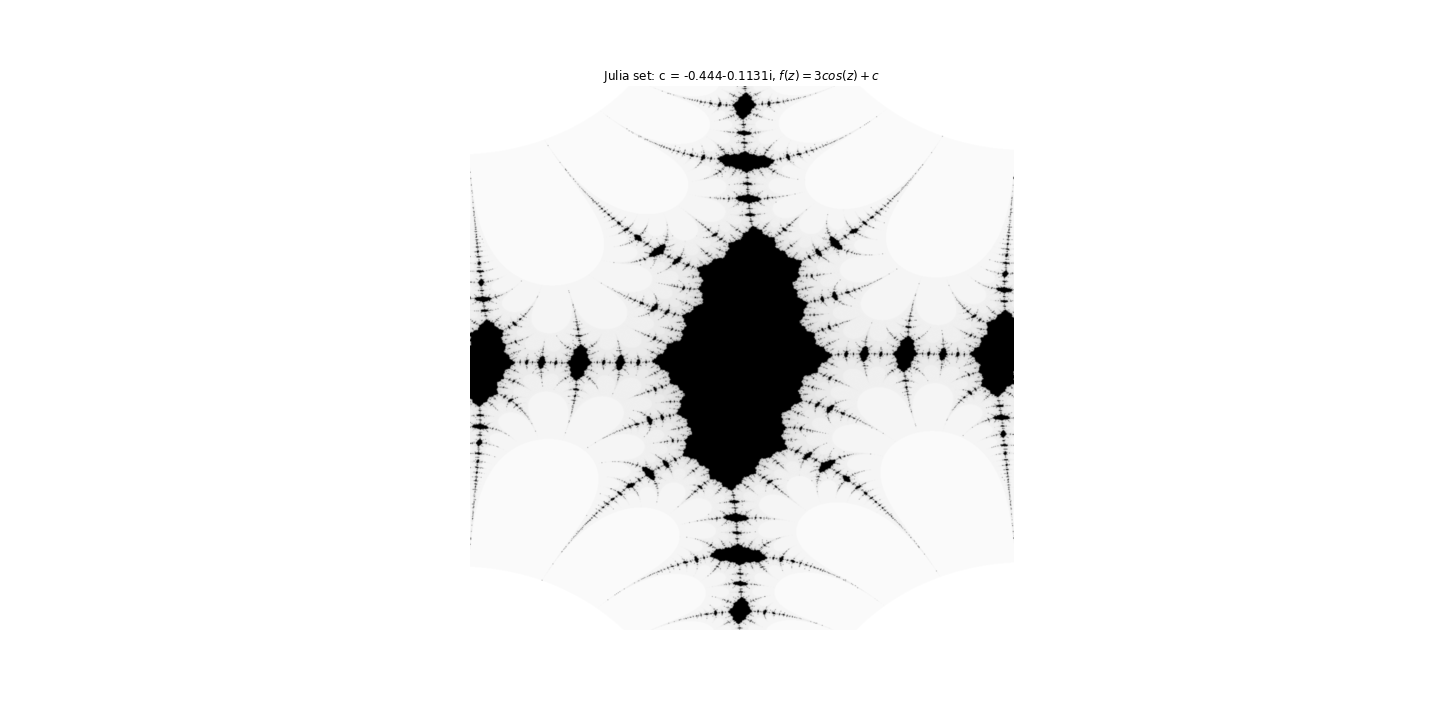
\includegraphics[width=\linewidth]{Fractal_image/3cos(z)+c_-0444+-01131.png}
  \end{subfigure}
  \begin{subfigure}[b]{1\linewidth}
    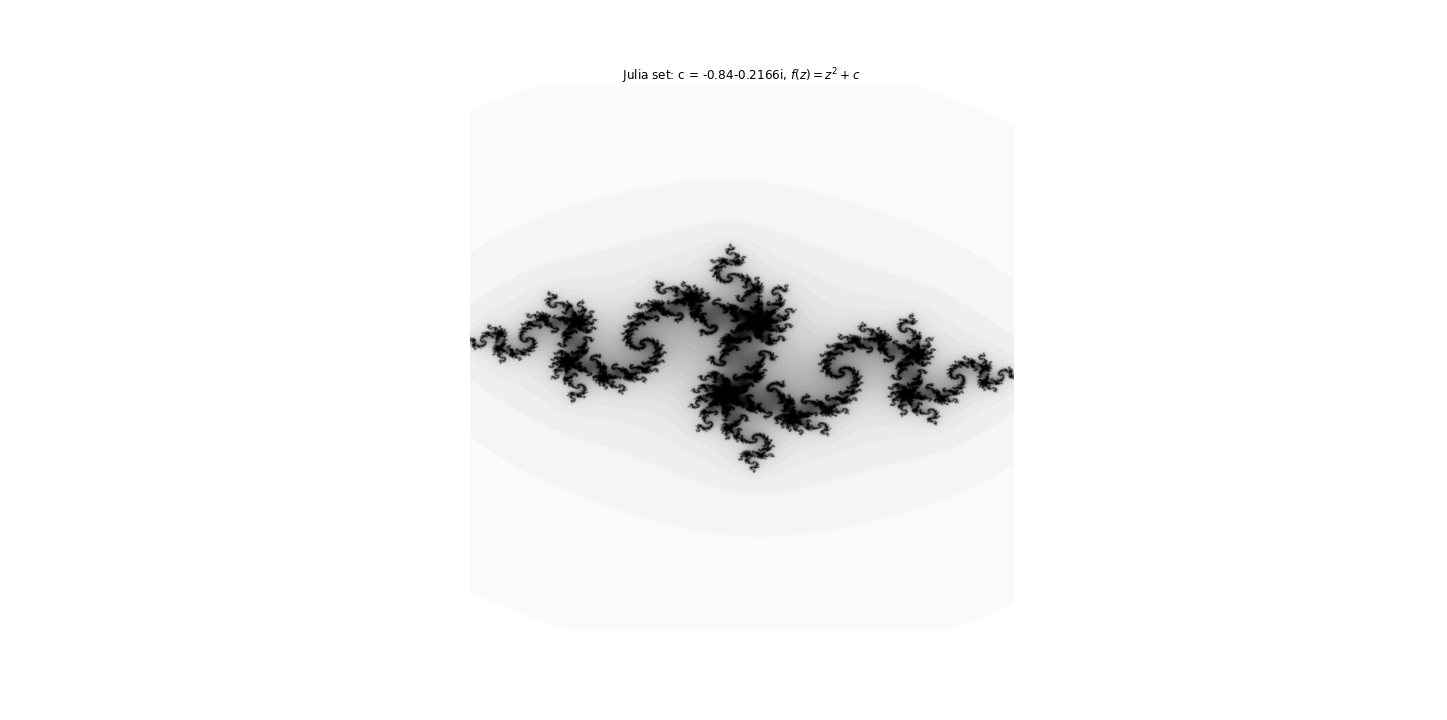
\includegraphics[width=\linewidth]{Fractal_image/z^2+c_-084+-02166.png}
  \end{subfigure}
\end{figure}

\newpage

\begin{figure}[h!]
  \centering
  \begin{subfigure}[b]{1\linewidth}
    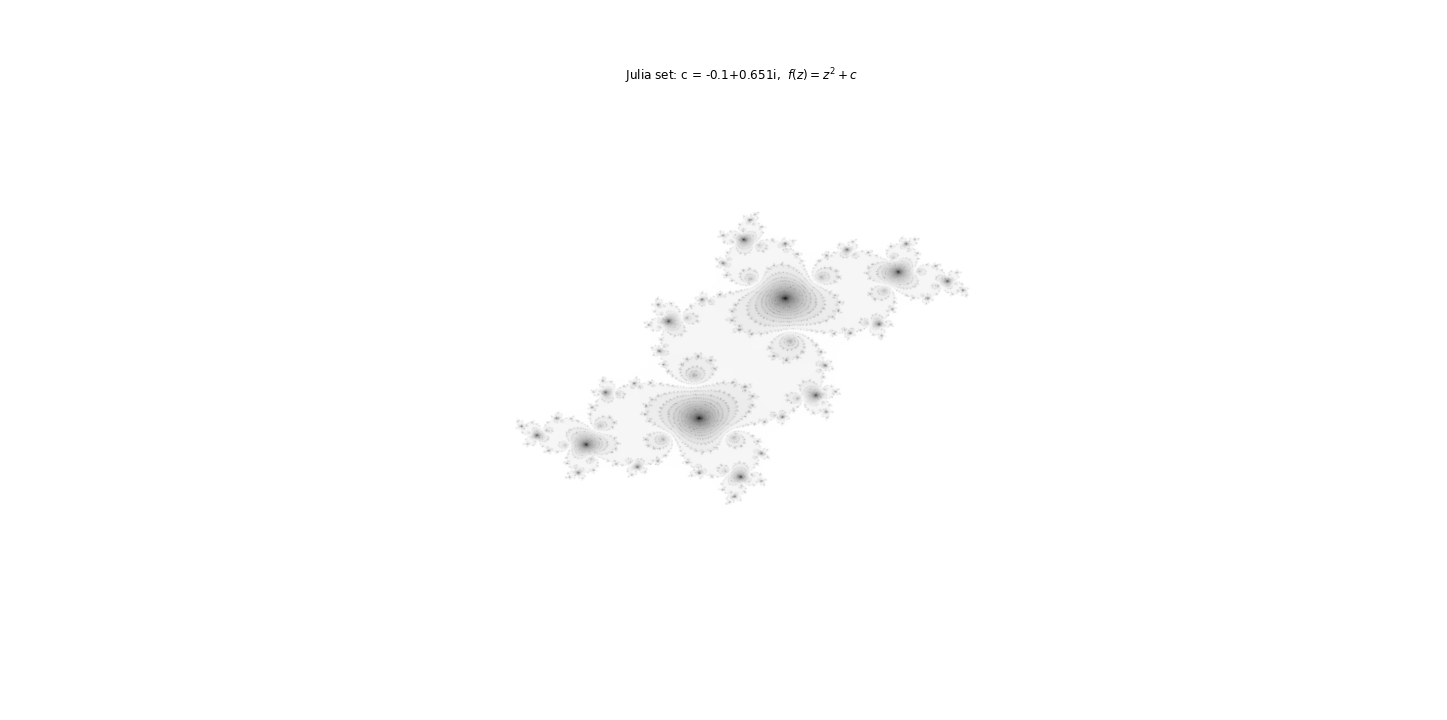
\includegraphics[width=\linewidth]{Fractal_image/z^2+c_-01+0651.png}
  \end{subfigure}
  \begin{subfigure}[b]{1\linewidth}
    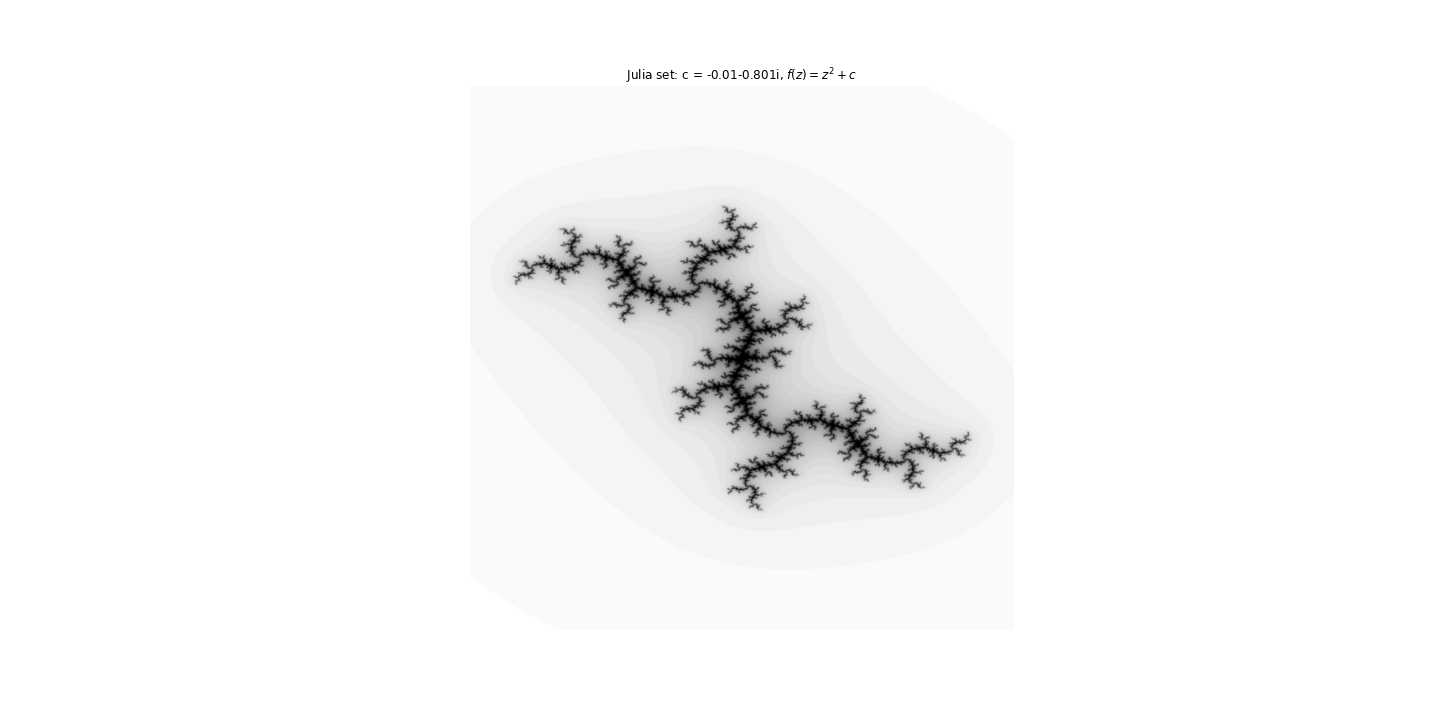
\includegraphics[width=\linewidth]{Fractal_image/z^2+c_-001+-0801.png}
  \end{subfigure}
\end{figure}

\newpage

\begin{figure}[h!]
  \centering
  \begin{subfigure}[b]{1\linewidth}
    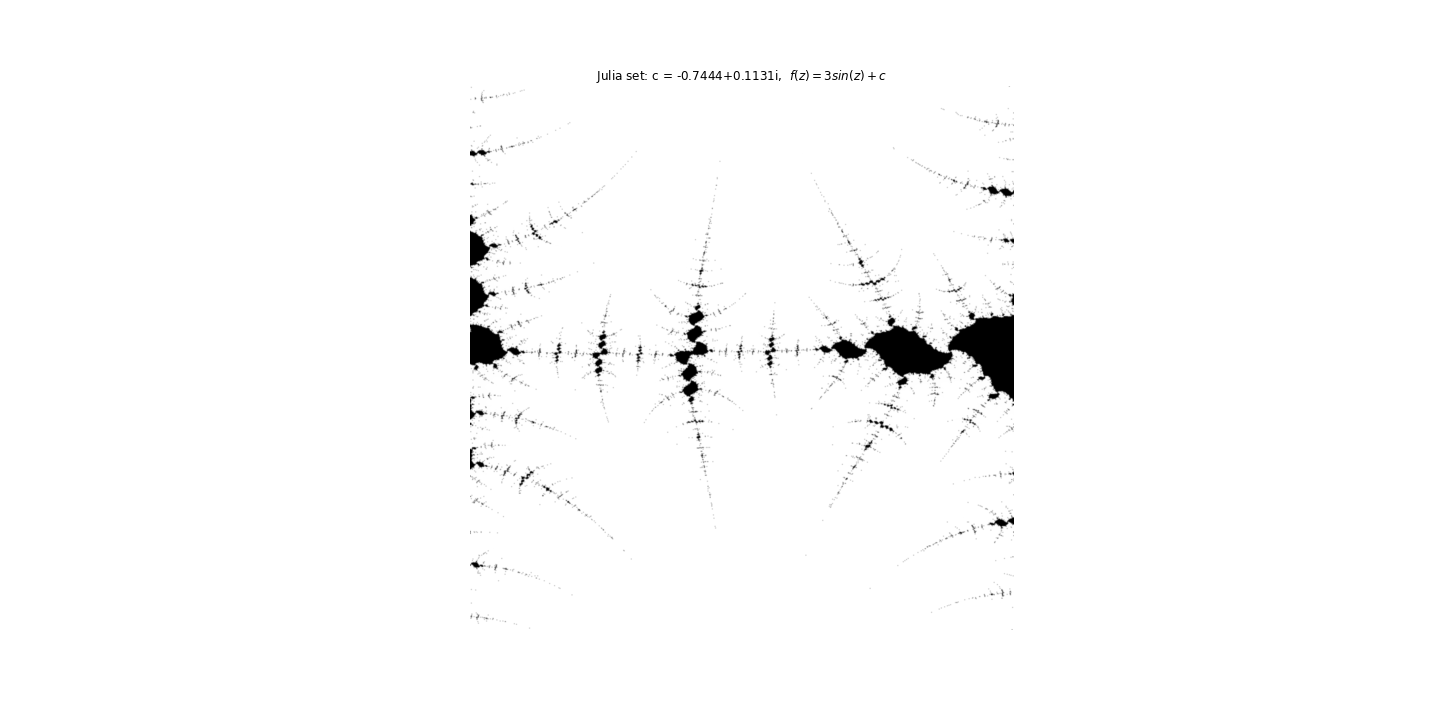
\includegraphics[width=\linewidth]{Fractal_image/3sin(z)+c_-07444+01131.png}
  \end{subfigure}
  \begin{subfigure}[b]{1\linewidth}
    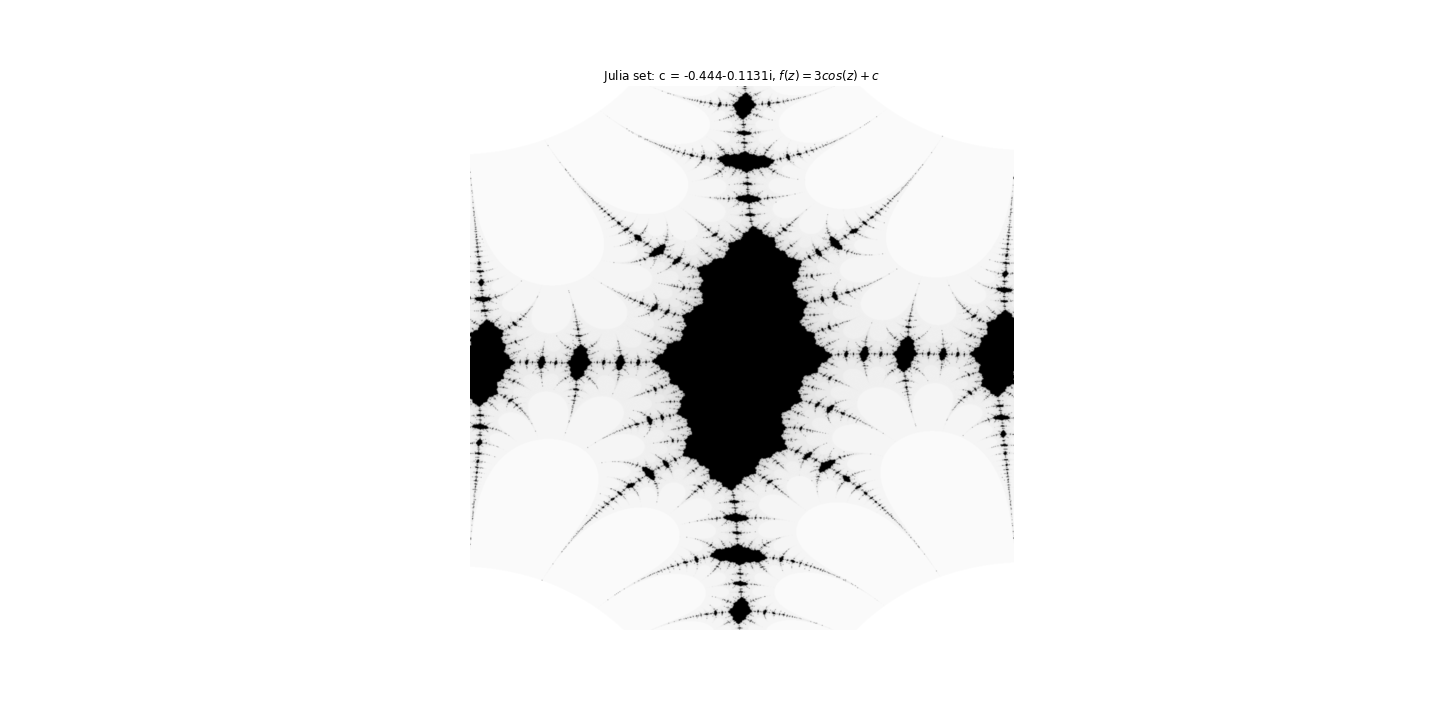
\includegraphics[width=\linewidth]{Fractal_image/3cos(z)+c_-0444+-01131.png}
  \end{subfigure}
\end{figure}

\newpage

\printbibliography[title = {References}]

\end{document}
